% File: SimpleBar.tex
% Author: Adam Leeper
%------------------------------------------------------------------------------
\providecommand{\isolatedBuild}[1]{#1}% Fallback definition to build normally.
\isolatedBuild{
  \documentclass[11pt,letterpaper]{book}
  %\documentclass[11pt,letterpaper]{book}

% aleeper: I think these are needed for Paul's macros?
\usepackage{epsfig}
\usepackage{epstopdf}

%\makeatletter
%\typeout{The import path is \import@path}
%\makeatother

\usepackage{import}

\subimport{./}{packagesMitiguy.sty}
\subimport{./}{macrosMitiguy.tex}
\subimport{./}{PageStylesMitiguy.tex}
\subimport{./}{macrosLeeper.tex}
   % Found via TEXINPUTS environment variable.
  \isolatedBuildHeader{Planar Rigid-Body Motion}
                      {Dynamics of a Swinging Bar}
}
%%%
%%%
%%%
A slender uniform slender rod of mass $m = 5$ kg and length $L = 2$ m is shown.
Gravity acts ``downward".
\begin{enumerate}
  \item Find a scalar differential equation of motion for $\theta$.
    Introduce additional identifiers as needed.
  \item With your result from (a), use the values given to compute the
    magnitude of the angular acceleration of the rod when $\theta = 0$ and
    when $\theta = \degrees{90}$.
\end{enumerate}

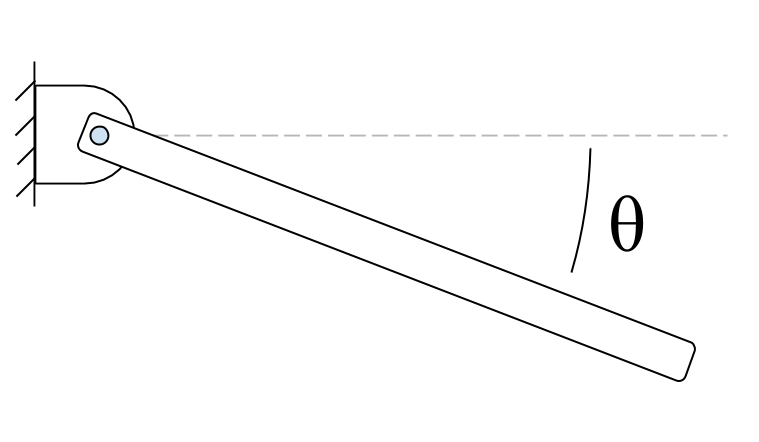
\includegraphics[width=0.35\textwidth]{SlenderRod_angle.png}
%
\isolatedBuildFooter
